\section*{ÔN TẬP CHƯƠNG II}
\subsection{CÂU TRẮC NGHIỆM NHIỀU PHƯƠNG ÁN LỰA CHỌN}
\textit{Thí sinh trả lời từ câu 1 đến câu 18. Mỗi câu hỏi thí sinh chọn một phương án}
\Opensolutionfile{ans}[ans/G12Y24B15TN]
% ===================================================================
\begin{ex}
Đường biểu diễn sự biến thiên của áp suất theo thể tích của một lượng khí lí tưởng nhất định ở hình vẽ bên mô tả quá trình nào?
\begin{center}
	\begin{tikzpicture}  
		\begin{axis}[  ultra thick,
			xmin=0,  
			xmax=24,  
			xtick=\empty,
			ytick=\empty,
			ymin=0,  
			ymax=5.8, 
			samples=300,
			xticklabels=\empty,
			yticklabels=\empty,
			axis lines=center, 
			xlabel=$V$, 
			ylabel=$p$, 
			every axis y label/.style={at=(current axis.above origin),anchor=south},  
			every axis x label/.style={at=(current axis.right of origin),anchor=west},  ] 
			\addplot [ultra thick, blue, smooth, domain=3:20] {15/x}; 
		\end{axis}  
		\node[label={[below left]90:O}] at (0,0){};
	\end{tikzpicture}
\end{center}
	\choice
	{Đẳng tích}
	{Đẳng entropy}
	{Đẳng áp}
	{\True Đẳng nhiệt}
	\loigiai{}
\end{ex}
% ===================================================================
\begin{ex}
	Đại lượng nào sau đây \textbf{không phải} là thông số trạng thái của một lượng khí?
	
	\choice
	{Thể tích}
	{Áp suất}
	{\True Khối lượng}
	{Nhiệt độ}
	\loigiai{}
\end{ex}
% ===================================================================
\begin{ex}
	Với $\Delta U$, $Q$, $A$ lần lượt là độ biến thiên nội năng hệ, nhiệt lượng và công hệ nhận thì công thức đúng của định luật I nhiệt động lực học là
	\choice
	{$\Delta U=A$}
	{$\Delta U=Q$}
	{$\Delta U=Q\cdot A$}
	{\True $\Delta U=Q+A$}
	\loigiai{}
\end{ex}
% ===================================================================
\begin{ex}
Phát biểu nào sau đây là đúng với nội dung định luật Boyle?	
	\choice
	{\True Trong quá trình đẳng nhiệt của một lượng khí nhất định, áp suất tỉ lệ nghịch với thể tích}
	{Trong quá trình đẳng áp của một khối lượng khí xác định, áp suất và thể tích là một hằng số}
	{Trong quá trình đẳng tích của một khối khí xác định, tích của áp suất và thể tích là một hằng số}
	{Trong quá trình đẳng nhiệt của một lượng khí nhất định, áp suất tỉ lệ thuận với thể tích}
	\loigiai{}
\end{ex}
% ===================================================================
\begin{ex}
	Hiện nay, nhiệt độ thấp nhất trong phòng thí nghiệm mà con người thực hiện được vào khoảng
	
	\choice
	{$\SI{-9}{\kelvin}$}
	{$\SI{-9}{\celsius}$}
	{\True $\SI{E-9}{\kelvin}$}
	{$\SI{E9}{\kelvin}$}
	\loigiai{}
\end{ex}
% ===================================================================
\begin{ex}
Điều nào sau đây là \textbf{sai} khi nói về mô hình động học phân tử chất khí?
	
	\choice
	{Chất khí được cấu tạo từ các nguyên tử, phân tử riêng biệt}
	{Các phân tử chuyển động hỗn loạn, không ngừng}
	{Các nguyên tử, phân tử tương tác với nhau bằng lực hút và lực đẩy}
	{\True Các phân tử luôn hút nhau để tạo thành chất}
	\loigiai{}
\end{ex}
% ===================================================================
\begin{ex}
	Hệ thức nào sau đây phù hợp với định luật Charles?
	\choice
	{$V\sim t$}
	{\True $\dfrac{V_1}{T_1}=\dfrac{V_2}{T_2}$}
	{$\dfrac{V}{t}=\text{hằng số}$}
	{$\dfrac{V_1}{V_2}=\dfrac{T_2}{T_1}$}
	\loigiai{}
\end{ex}
% ===================================================================
\begin{ex}
	Trong quá trình đẳng tích thì áp suất của một lượng khí xác định
	\choice
	{tỉ lệ thuận với bình phương của nhiệt độ tuyệt đối}
	{\True tỉ lệ thuận với nhiệt độ tuyệt đối}
	{tỉ lệ thuận với căn bậc hai của nhiệt độ tuyệt đối}
	{tỉ lệ nghịch với nhiệt độ}
	\loigiai{}
\end{ex}
% ===================================================================
\begin{ex}
Chọn đáp án \textbf{đúng}. Nội năng của một vật là
	\choice
	{tổng động năng và thế năng của vật.  }
	{tổng nhiệt lượng và cơ năng mà vật nhận được trong quá trình truyền nhiệt và thực hiện công}
	{\True tổng động năng và thế năng của các phân tử cấu tạo nên vật}
	{nhiệt lượng vật nhận được trong quá trình truyền nhiệt}
	\loigiai{}
\end{ex}
% ===================================================================
\begin{ex}
Chọn phát biểu \textbf{không đúng}.\\
Nung nóng đẳng nhiệt một lượng khí lí tưởng chứa trong cylanh có piston di chuyển được thì
	
	\choice
	{nhiệt lượng bằng không vì nhiệt được của khí không đổi}
	{\True nội năng của khí bằng không vì nhiệt độ của khí không thay đổi}
	{nhiệt lượng mà khí nhận được chuyển hết sang công mà khí sinh ra}
	{nội năng của lượng khí không thay đổi}
	\loigiai{}
\end{ex}
% ===================================================================
\begin{ex}
	Khi đun nóng đẳng tích khối khí lí tưởng thêm $\SI{1}{\celsius}$ thì áp suất khối khí tăng thêm $\dfrac{1}{360}$ áp suất ban đầu. Nhiệt độ ban đầu của khối khí đó là 
	\choice
	{\True $\SI{87}{\celsius}$}
	{$\SI{360}{\celsius}$}
	{$\SI{350}{\celsius}$}
	{$\SI{361}{\celsius}$}
	\loigiai{\begin{center}
			\begin{tabular}{C{4cm} C{3cm} C{4cm}}
				\colorbox{yellow}{\textcolor{red}{\textbf{Trạng thái 1}}} & $\xrightarrow[]{V=\text{const}}$ & \colorbox{yellow}{\textcolor{red}{\textbf{Trạng thái 2}}}\\
				$p_1=p$ & &$p_2=\left(1+\dfrac{1}{360}\right)P$\\
				$T_1=?$ & & $T_2=T_1+1$
			\end{tabular}
		\end{center}
		$$\dfrac{T_1}{p_1}=\dfrac{T_2}{p_2}\Leftrightarrow \dfrac{T_1}{p}=\dfrac{T_1+1}{p\left(1+\dfrac{1}{360}\right)}\Rightarrow T_1=\SI{360}{\kelvin}\Rightarrow t_1=\SI{87}{\celsius}.$$
	}
\end{ex}
% ===================================================================
\begin{ex}
Nén khí đẳng nhiệt từ thể tích $\SI{10}{\liter}$ xuống còn thể tích $\SI{4}{\liter}$ thì áp suất khí tăng lên
	
	\choice
	{\True 2,5 lần}
	{2 lần}
	{1,5 lần}
	{4 lần}
	\loigiai{$$\dfrac{p_2}{p_1}=\dfrac{V_1}{V_2}=2,5.$$
	}
\end{ex}
% ===================================================================
\begin{ex}
Một khối khí lí tưởng nhốt trong bình kín. Tăng nhiệt độ của khối khí từ $\SI{100}{\celsius}$ lên $\SI{200}{\celsius}$ thì áp suất trong bình sẽ
	
	\choice
	{có thể tăng hoặc giảm}
	{tăng lên hơn 2 lần áp suất cũ}
	{\True tăng lên ít hơn 2 lần áp suất cũ}
	{tăng lên đúng bằng 2 lần áp suất cũ}
	\loigiai{}
\end{ex}
% ===================================================================
\begin{ex}
	Khi làm nóng một lượng khí trong bình kín thì
	\choice
	{số phân tử khí trong một đơn vị thể tích giảm tỉ lệ nghịch với nhiệt độ tuyệt đối}
	{\True áp suất khí không đổi}
	{số phân tử khí trong một đơn vị thể tích không đổi}
	{số phân tử khí trong một đơn vị thể tích tăng tỉ lệ với nhiệt độ tuyệt đối}
	\loigiai{}
\end{ex}
% ===================================================================
\begin{ex}
Nung nóng đẳng áp khối khí lí tưởng từ nhiệt độ $\SI{27}{\celsius}$ đến $\SI{177}{\celsius}$ thì thể tích khí tăng một lượng $\Delta V=\SI{3}{\liter}$. Thể tích ban đầu của khí đó là	
	\choice
	{$\SI{3}{\liter}$}
	{$\SI{4.5}{\liter}$}
	{\True $\SI{6}{\liter}$}
	{$\SI{9}{\liter}$}
	\loigiai{$$\dfrac{V_1}{T_1}=\dfrac{V_2}{T_2}\Leftrightarrow \dfrac{V_1}{27+273}=\dfrac{V_1+3}{177+273}\Rightarrow V_1=\SI{6}{\liter}.$$
	}
\end{ex}
% ===================================================================
\begin{ex}
Trong một động cơ diesel, khối khí có nhiệt độ ban đầu là $\SI{32}{\celsius}$ được nén để thể tích bằng $1/16$ thể tích ban đầu và áp suất tăng bằng 48,5 lần áp suất ban đầu. Nhiệt độ khối khí sau khi nén sẽ \textbf{gần nhất} với giá trị nào sau đây?
	
	\choice
	{\True $\SI{652}{\celsius}$}
	{$\SI{97}{\celsius}$}
	{$\SI{1552}{\celsius}$}
	{$\SI{132}{\celsius}$}
	\loigiai{\begin{center}
			\begin{tabular}{C{4cm} C{3cm} C{4cm}}
				\colorbox{yellow}{\textcolor{red}{\textbf{Trạng thái 1}}} & $\xrightarrow[]{\nu=\text{const}}$ & \colorbox{yellow}{\textcolor{red}{\textbf{Trạng thái 2}}}\\
				$p_1$ & &$p_2=48,5p_1$\\
				$V_1$ & & $V_2=V_1/16$\\
				$T_1=\SI{305}{\kelvin}$ & & $T_2=?$
			\end{tabular}
		\end{center}
		$$\dfrac{p_1V_1}{T_1}=\dfrac{p_2V_2}{T_2}\Rightarrow T_2=\SI{924.5}{\kelvin}\Rightarrow t_2=\SI{652}{\celsius}.$$
	}
\end{ex}
% ===================================================================
\begin{ex}
Hình bên là đồ thị mô tả sự biến đổi trạng thái của một lượng khí lí tưởng trong hệ toạ độ $\left(V, T\right)$. Đồ thị của sự biến đổi trạng thái trên trong hệ toạ độ $\left(p, T\right)$ tương ứng với hình nào?
\begin{center}
	\includegraphics[width=0.2\linewidth]{figs/VN12-Y24-PH-SYL-016-7}
\end{center}
\begin{center}
	\includegraphics[width=0.9\linewidth]{figs/VN12-Y24-PH-SYL-016-8}
\end{center}
	
	\choice
	{Hình a}
	{Hình b}
	{Hình c}
	{\True Hình d}
	\loigiai{}
\end{ex}
% ===================================================================
\begin{ex}
	Một mẫu khí lí tưởng biến đổi từ trạng thái đầu $a$ tới trạng thái cuối $b$ theo ba quá trình khác nhau như mô tả trên hình vẽ. Nhiệt lượng cung cấp cho mẫu khí trong quá trình (1) là $10p_iV_i$. Kết luận nào sau đây \textbf{đúng}?
	\begin{center}
		\includegraphics[width=0.45\linewidth]{figs/VN12-Y24-PH-SYL-016-6}
	\end{center}
	\begin{center}
		\begin{tabular}{|C{2cm}|C{7cm}|C{7cm}|}
			\hline
			& \thead{Nhiệt lượng cung cấp cho\\ chất khí trong quá trình (2)} &\thead{Độ biến thiên nội năng của\\ chất khí trong quá trình (3)}\\
			\hline
			Kết luận 1 & $3p_iV_i$ & $-3p_iV_i$\\
			\hline
			Kết luận 2 & $2p_iV_i$ & $-2p_iV_i$\\
			\hline
			Kết luận 3 & $2p_iV_i$ & $-3p_iV_i$\\
			\hline
			Kết luận 4 & $11p_iV_i$ & $6p_iV_i$\\
			\hline
		\end{tabular}
	\end{center}
	\choice
	{Kết luận 1}
	{Kết luận 2}
	{Kết luận 3}
	{\True Kết luận 4}
	\loigiai{Công khí thực hiện trong quá trình (1) là $A'_1=p_i\left(5V_i-V_i\right)=4p_iV_i.$\\
		Công khí thực hiện trong quá trình (2) là $A'_2=\dfrac{1}{2}\left(1,5p_i+p_i\right)\left(5V_i-V_i\right)=5p_iV_i$.\\
		Độ biến thiên nội năng của khối khí trong 3 quá trình là như nhau.
		$$\Delta U=Q_1-A'_1=10p_iV_i-4p_iV_i=6p_iV_i.$$
		$$Q_2=\Delta U+A'_2=11p_iV_i.$$
	}
\end{ex}
\Closesolutionfile{ans}
\subsection{CÂU TRẮC NGHIỆM ĐÚNG/SAI}
\textit{Thí sinh trả lời từ câu 1 đến câu 4. Trong mỗi ý \textbf{a)}, \textbf{b)}, \textbf{c)}, \textbf{d)} ở mỗi câu, thí sinh chọn đúng hoặc sai}
\setcounter{ex}{0}
% ===================================================================
\begin{ex}
	Một khối khí lí tưởng thực hiện quá trình biến đổi trạng thái như hình vẽ bên. Thể tích ban đầu của khối khí ở trạng thái (1) là $\SI{12}{\liter}$.
	\begin{center}
		\includegraphics[width=0.45\linewidth]{figs/VN12-Y24-PH-SYL-016-2}
	\end{center}
	\begin{enumerate}[label=\alph*)]
		\item Quá trình $(1) - (2)$ khối khí biến đổi đẳng nhiệt.
		\item Quá trình từ $(2) - (3)$ khối khí biến đổi đẳng áp.
		\item Thể tích khí ở trạng thái (3) là $\SI{18}{\liter}$.
		\item Số mol khí là $\SI{1.95}{\mole}$.
	\end{enumerate}
	\loigiai{\begin{enumerate}[label=\alph*)]
			\item Sai. $(1)-(2)$ là quá trình đẳng tích.
			\item Đúng.
			\item Đúng.
			\item Đúng.
		\end{enumerate}
	}
\end{ex}
% ===================================================================
\begin{ex}
	Bóng thám không có các bộ phận chính như mô tả ở hình bên.
	\begin{center}
		\includegraphics[width=0.3\linewidth]{figs/VN12-Y24-PH-SYL-016-3}
	\end{center}
	\begin{enumerate}[label=\alph*)]
		\item Vỏ bóng được làm từ chất liệu đàn hồi.
		\item Khí bơm vào bóng phải có khối lượng riêng lớn hơn khối lượng riêng của không khí.
		\item Thông thường bóng chỉ bay lên tới độ cao $\SI{30}{\kilo\meter}$ đến $\SI{40}{\kilo\meter}$ là bị vỡ vì càng lên cao áp suất khí bên ngoài càng tăng và ép vỡ bóng.
		\item Sau khi bóng vỡ, hộp đựng thiết bị và dù sẽ rơi nhanh dần đều xuống mặt đất.
	\end{enumerate}
	
	\loigiai{\begin{enumerate}[label=\alph*)]
			\item Đúng.
			\item Sai. Khối lượng riêng khí bơm vào nhỏ hơn khối lượng riêng của không khí để lực nâng của không khí tác dụng lên bóng lớn hơn trọng lực của bóng và dụng cụ.
			\item Sai. Càng lên cao áp suất càng giảm do đó thể tích khí trong bóng tăng dần làm cho vỏ bóng dãn ra.
			\item Sai. Trong quá trình rơi, dù và hộp thiết bị chịu tác dụng của trọng lực và lực cản của không khí. Ban đầu chúng chuyển động nhanh dần đều, sau đó lực cản tăng lên nên chúng chuyển động nhanh dần nhưng không đều, khi lực cản có độ lớn bằng trọng lực thì chúng chuyển động đều.
		\end{enumerate}
	}
\end{ex}
% ===================================================================
\begin{ex}
Một khối khí lí tưởng đã thực hiện chu trình biến đổi trạng thái như đồ thị hình bên dưới.
\begin{center}
	\includegraphics[width=0.4\linewidth]{figs/VN12-Y24-PH-SYL-016-4}
\end{center}
\begin{enumerate}[label=\alph*)]
	\item Có 2 quá trình biến đổi đẳng tích.
	\item Quá trình biến đổi $(4) - (1)$ là quá trình nén đẳng áp.
	\item Độ biến thiên nội năng của khí trong chu trình bằng 0.
	\item Trạng thái (3) có thể tích lớn nhất.
\end{enumerate}	
	\loigiai{\begin{enumerate}[label=\alph*)]
			\item Sai. Có 1 quá trình đẳng tích là $(1)-(2)$.
			\item Đúng. Quá trình $(4)-(1)$ là quá trình đẳng áp nhiệt độ giảm $\rightarrow$ thể tích giảm.
			\item Đúng. Chu trình kín thì $\Delta U=0$.
			\item Sai. Trạng thái (4) có thể tích lớn nhất.
			\begin{center}
				\includegraphics[width=0.5\linewidth]{figs/VN12-Y24-PH-SYL-016-5}
			\end{center}
			$p_A=p_B=p_C $ mà $T_C>T_B>T_A\Rightarrow V_C>V_B>V_A\Rightarrow V_4>V_3>V_2=V_1$.
		\end{enumerate}
	}
\end{ex}
% ===================================================================
\begin{ex}
	Một bình kín có dung tích $\SI{10}{\liter}$ chứa một khối khí lí tưởng đơn nguyên tử ở áp suất $p=\SI{380}{\milli\meter Hg}$. Nhiệt độ khối khí là $\SI{10.0}{\celsius}$. 
	\begin{enumerate}[label=\alph*)]
		\item Mật độ phân tử khí là $\SI{9.7E22}{\meter^{-3}}$.
		\item Động năng trung bình của phân tử khí là $\SI{5.86E-21}{\joule}$.
		\item Nội năng khí chứa trong bình là $\SI{759.75}{\joule}$.
		\item Nếu người ta mở nắp bình trong môi trường có nhiệt độ $\SI{10}{\celsius}$ và áp suất bằng $\SI{760}{\milli\meter Hg}$ thì số phân tử khí trong bình giảm xuống.
	\end{enumerate}
	
	\loigiai{\begin{enumerate}[label=\alph*)]
			\item Sai.
			$$\mu=\dfrac{p}{kT}=\dfrac{\left(\SI{380}{\milli\meter Hg}\right)\cdot\left(\SI{1.013E5}{\pascal}\right)}{\left(\SI{760}{\milli\meter Hg}\right)\cdot\left(\SI{1.38E-23}{\joule/\kelvin}\right)\cdot\left(\SI{283}{\kelvin}\right)}\approx\SI{1.3E25}{\meter^{-3}}.$$
			\item Đúng.
			\item Đúng.
			$$U=\dfrac{3}{2}n RT=\dfrac{3}{2}pV=\SI{759.75}{\joule}.$$
			\item Sai.
			$$N=\dfrac{pVN_A}{RT}.$$
			Khi mở nắp bình, áp suất khí trong bình tăng nên $N$ tăng.
		\end{enumerate}
	}
\end{ex}
\subsection{CÂU TRẮC NGHIỆM TRẢ LỜI NGẮN}
\textit{Thí sinh trả lời từ câu 1 đến câu 6}
\setcounter{ex}{0}
% ===================================================================
\begin{ex}
	Một cái bơm chứa $\SI{100}{\centi\meter^3}$ không khí ở nhiệt độ $\SI{27}{\celsius}$ ở áp suất $\SI{E5}{\pascal}$. Khi không khí bị nén xuống còn $\SI{20}{\centi\meter^3}$ và nhiệt độ tăng lên tới $\SI{327}{\celsius}$ thì áp suất của không khí trong bơm lúc này là bao nhiêu \textit{(tính theo đơn vị $\SI{E5}{\pascal}$ )}.
	\loigiai{$$\dfrac{p_1V_1}{T_1}=\dfrac{p_2V_2}{T_2}\Rightarrow p_2=\SI{10E5}{\pascal}.$$	
	}
\end{ex}
% ===================================================================
\begin{ex}
	Một bình kín thể tích $\SI{0.5}{\meter^3}$ chứa không khí ở nhiệt độ $\SI{32}{\celsius}$ và áp suất $\SI{1.3}{atm}$. Khi mở nắp bình, áp suất không khí còn lại là $\SI{1}{atm}$ và nhiệt độ $\SI{0}{\celsius}$. Thể tích không khí thoát ra khỏi bình là bao nhiêu lít \textit{(làm tròn đến 2 chữ số thập phân)}?
	
	\loigiai{$$\dfrac{p_1V_1}{T_1}=\dfrac{p_2V_2}{T_2}\Rightarrow V_2=\SI{581.80}{\liter}\Rightarrow \Delta V=\SI{81.80}{\liter}.$$
	}
\end{ex}
% ===================================================================
\begin{ex}
	Một bình dung tích $\SI{10}{\liter}$ chứa $\SI{1}{\mole}$ khí helium ở áp suất $\SI{2.5}{atm}$. Động năng trung bình của phân tử khí trong bình là bao nhiêu \textit{(tính theo đơn vị $\SI{E-21}{\joule}$ và làm tròn đến 2 chữ số thập phân)}. 
	
	\loigiai{$$p=\dfrac{2}{3}\mu W_\text{đ}=\dfrac{2}{3}\cdot\dfrac{n N_A}{V}\cdot W_\text{đ}$$
		$$\Rightarrow W_\text{đ}=\dfrac{3}{2}\cdot\dfrac{pV}{n N_A}\approx\SI{6.31E-21}{\joule}.$$}
\end{ex}
% ===================================================================
\begin{ex}
Một căn phòng có thể tích $\SI{40}{\meter^3}$. Không khí trong phòng có nhiệt độ $\SI{27}{\celsius}$ và ở áp suất $\SI{1}{atm}$. Số phân tử khí trong phòng là $\xsi{x\cdot10^{26}}{\text{phân tử}}$. Xác định giá trị của $x$ \textit{(làm tròn đến 2 chữ số thập phân)}?
	
	\loigiai{$$p=nkT=\dfrac{NkT}{V}\Rightarrow N=\dfrac{pV}{kT}\approx\SI{9.79E26}{\text{phân tử}}.$$}
\end{ex}
% ===================================================================
\begin{ex}
	Một khối khí $\ce{CO_2}$ có khối lượng $m=\SI{250}{\gram}$ chứa trong một cylanh dưới piston nặng. Piston có thể di chuyển không ma sát, thẳng đứng theo thành của cylanh. Đun nóng từ từ cylanh cho nhiệt độ tăng từ $t_1=\SI{27}{\celsius}$ lên $\SI{127}{\celsius}$. Tính công do khí thực hiện theo đơn vị $\si{\kilo\joule}$ \textit{(làm tròn đến 2 chữ số thập phân)}.
	
	\loigiai{$$A'=p\left(V_2-V_1\right)=\dfrac{m}{\mu}R\left(T_2-T_1\right)\approx\SI{4.72}{\kilo\joule}.$$
	}
\end{ex}
% ===================================================================
\begin{ex}
	Một lượng khí lí tưởng đơn nguyên tử chuyển từ trạng thái (1) sang trạng thái (2) bằng hai cách:
	\begin{itemize}
		\item Cách 1: $(1)\rightarrow (3)\rightarrow (2)$.
		\item Cách 2: $(1)\rightarrow(4)\rightarrow (2)$.
	\end{itemize}
	\begin{center}
		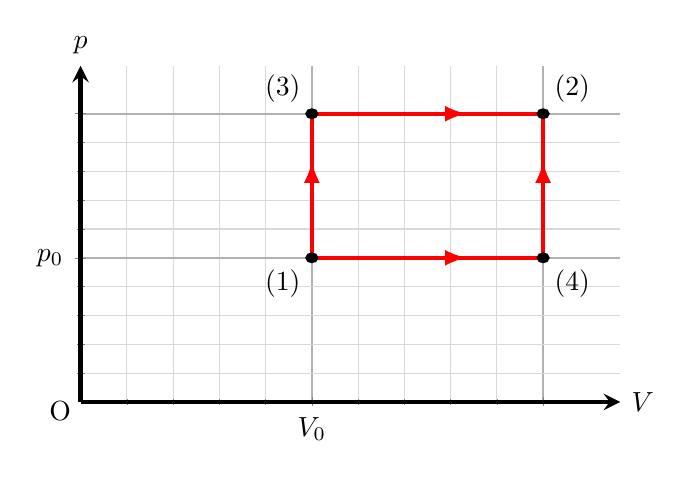
\begin{tikzpicture}  
			\begin{axis}[  ultra thick, yscale=0.75,
				xmin=0,  
				xmax=7,  
				ytick={0,3,6},
				xtick={0,3,6},
				ymin=0,  
				ymax=7, 
				samples=300,
				yticklabels={,$p_0$,},
				xticklabels={,$V_0$,},
				axis lines=center, 
				xlabel=$V$, 
				ylabel=$p$, 
				every axis y label/.style={at=(current axis.above origin),anchor=south},  
				every axis x label/.style={at=(current axis.right of origin),anchor=west},
				minor x tick num=4,
				minor y tick num=4,
				grid style={step=1, line width =0.4pt, color=gray!30!white},
				grid=both,
				major grid style={line width=0.8pt,gray!60!white},
				]
				\draw[ultra thick, red] (axis cs: 3, 3) -- (axis cs:6, 3);
				\draw[ultra thick,-latex, red] (axis cs: 3, 3) -- (axis cs: 5, 3);
				\draw[ultra thick, red] (axis cs: 3, 6) -- (axis cs:6, 6);
				\draw[ultra thick,-latex, red] (axis cs: 3, 6) -- (axis cs: 5, 6);
				\draw[ultra thick, red] (axis cs: 3, 3) -- (axis cs:3, 6);
				\draw[ultra thick,-latex, red] (axis cs: 3, 3) -- (axis cs: 3, 5);
				\draw[ultra thick, red] (axis cs: 6, 3) -- (axis cs:6, 6);
				\draw[ultra thick,-latex, red] (axis cs: 6, 3) -- (axis cs: 6, 5);
				
				\filldraw[black] (axis cs:3,3) circle (1.5pt) node[below left] {(1)};
				\filldraw[black] (axis cs:6,6) circle (1.5pt) node[above right] {(2)};
				\filldraw[black] (axis cs:3,6) circle (1.5pt) node[above left] {(3)};
				\filldraw[black] (axis cs:6,3) circle (1.5pt) node[below right] {(4)};
			\end{axis}  
			\node[label={[below left]90:O}] at (0,0){};
		\end{tikzpicture}
	\end{center}
	Hãy tìm tỉ số các nhiệt lượng cần truyền cho khí trong cách 1 và cách 2 \textit{(làm tròn đến 2 chữ số thập phân)}.
	
	\loigiai{Độ biến thiên nội năng khi chuyển từ trạng thái (1) sang (2):
		$$\Delta U=\dfrac{3}{2}\nu R\Delta T=\dfrac{3}{2}\cdot\left(p_2V_2-p_1V_1\right)=\dfrac{9}{2}p_0V_0.$$
		Công khí thực hiện trong cách 1:
		$$A'_1=2p_0V_0.$$
		Công khí thực hiện trong cách 2:
		$$A'_2=p_0V_0.$$
		Nhiệt lượng khí nhận:
		$$Q=\Delta U-A=\Delta U+A'$$
		$$\Rightarrow \dfrac{Q_1}{Q_2}=\dfrac{\dfrac{9}{2}p_0V_0+2p_0V_0}{\dfrac{9}{2}p_0V_0+p_0V_0}=\dfrac{13}{11}\approx1,18.$$
	}
\end{ex}